\documentclass[12pt, letter]{article}
\usepackage{amsfonts}
\usepackage{amssymb}
\usepackage{amsthm}
\usepackage{amsmath}
\usepackage{graphicx}
\usepackage{multicol}
\usepackage{pifont}
\usepackage{multirow}

\hfuzz2pt % Don't bother to report over-full boxes if over-edge is < 2pt

\newcommand{\zag}[1]{\left(#1\right)}
\newcommand{\zagv}[1]{\left\{#1\right\}}
\newcommand{\zags}[1]{\left[#1\right]}
\def\ffrac#1/#2{\leavevmode\kern-.2em
  \raise.5ex\hbox{ $\textstyle #1$}\kern-.05em
  /\kern-.35em\lower.25ex\hbox{ $\textstyle #2$}}
\newcommand{\abs}[1]{\left\vert#1\right\vert}
\newcommand{\DS}{\displaystyle}
\newcommand{\SSS}{\scriptstyle}
\newcommand{\TS}{\textstyle}
\newcommand{\tg}{\mathrm{tg}\,}
\newcommand{\deo}[1]{\textbf{\textsf #1}}
\newcounter{zad}
\newcommand{\problem}[1]{{\setcounter{zad}{171}
\addtocounter{zad}{#1}\bigskip
\hskip -22pt\Huge{\ding{\value{zad}}}\hskip 0pt}}
\newcommand{\arctg}{\mathrm{arctg}\,}
\newcommand{\A}{\alpha}
\newcommand{\R}{\mathbb{R}}
\newcommand{\set}[1]{\left\{#1\right\}}
\newcommand{\slika}[1]{\
\vskip-0mm\includegraphics[width=3.5in]{#1}\vskip 5mm\ }
\newcommand{\slikav}[1]{\
\vskip-25mm \ \\
\begin{center}\includegraphics[width=175mm]{#1}\end{center}\vskip-10mm\ }
\newcommand{\tekst}[1]{\vfill #1 \vfill}
\newcommand{\opis}[2]{\small{\textbf{Figure.#1}\\ #2}}
\newenvironment{prob}{ }{\ }
\newcommand{\mat}[2][rrrrrrrrrrrrrrrrrrrrrrrrrrrrrrrrrrrrrr]{\left[
    \begin{array}{#1}
    #2\\
    \end{array}
    \right]}

\newcounter{zadatak}
\newcommand{\z}{\addtocounter{zadatak}{1} \hskip -14pt {{%
{\textbf{\arabic{zadatak}.}}}}\hskip 5pt}



\textheight 215mm \textwidth 155mm
\hoffset -10mm \voffset -20mm
\pagestyle{empty} \parindent 0pt \parskip 8pt

        
        
\begin{document}

 \begin{center}
 {\Large Estimating the evolution of scoring rates in soccer match: \\ Model selection and variable
 selection  with ???-LASSO}\\[1cm]
 {Mladen Laudanovic and Frank Wood}
 \end{center}
 

% % !TEX root = deplump.tex
\subsection*{Abstract}

We present a general-purpose, lossless compressor for {\em streaming} data.  This compressor is based on a probabilistic, general-purpose, lossless compressor for {\em batch} data called deplump.  We both introduce a new approximation to inference in the probabilistic model underlying deplump and combine for the first time two existing approximations that together yield the computational asymptotics for inference required for streaming compresion.  We leave the name of the resulting streaming compressor the same, deplump, and demonstrate its performance on large text corpora.

%% !TEX root = main.tex
\section{Introduction}
\label{sec:introduction}

%Deplump \citep{Gasthaus2010} is a general purpose, lossless, batch compressor based on a probabilistic model of discrete sequences called the sequence memoizer \citep{Wood2009}.   \citeauthor{Gasthaus2010} showed that although deplump is algorithmically similar to the PPM and CTW compression algorithms, particularly their unbounded context lengths variants \citep{Cleary1997,Willems1998}, the coherent probabilistic model underlying deplump gives it a consistent empirical advantage.  In particular, \citeauthor{Gasthaus2010} showed that deplump generally outperformed CTW  \citep{Willems2009}, PPMZ \citep{Peltola2002}, and PPM* \citep{Cleary1997} on the large Calgary corpus, the Canterbury corpus, Wikipedia, and Chinese text.  Deplump was shown to underperform in comparison to the PAQ family of compressors \citep{Mahoney2005}, but the point was made that deplump (or more specifically the sequence memoizer) could replace one or all of the mixed, finite-order Markov-model predictors included in PAQ.  

The sequence memoizer \citep{Wood2009, Wood-2011-CACM} (SM) is a Bayesian nonparametric model for sequential stochastic processes that generate discrete observations.  Because the SM is a model in which the data is the sufficient statistic, it has space complexity that grows linearly as a function of the number of observations.  Since it was first introduced, two complementary modifications to the sequence memoizer have emerged \citep{Bartlett2010,Gasthaus2011} that, when combined as they were in \citep{Bartlett-2011-DCC}, together result in a constant space approximation to the sequence memoizer.  %Practically speaking, these approximations result in a model capable of actually incorporating streaming observations while still being representable on a fixed capacity computer.  

To review: the SM can be thought of as a hierarchical smoothing prior for multiple simultaneous conditional distribution estimation. 
% It can also, for instance, be viewed as a smoothing $n$-gram model in the limit of $n\rightarrow\infty$. 
 ``Observations'' in the SM are the discrete (countable) symbols generated by some underlying stochastic process and situated in the full sequence or ``context'' of observations that were already generated.  It has been shown that the space complexity of the sequence memoizer is on the order of the number of nodes in a suffix-tree representation of this sequence of observations times the storage required to represent the conditional density estimate at each node. An approximation to the sequence memoizer in which the number of nodes in the suffix-tree remains of asymptotically constant order was introduced in \citep{Bartlett2010}.  Unfortunately, in that work the storage requirement at each node grew as an uncharacterized but not-constant function of the input sequence length.  A method for constraining the memory to be of constant order at each node was later introduced in \citep{Gasthaus2011}.  Unfortunately, the representation they proposed resulted in the computational cost of inference growing as a super-linear function of the length of the training sequence.  \cite{Bartlett-2011-DCC} combined both and introduced two more approximations that rendered the computational cost of inference asymptotically linear in the observation sequence length and cost of storage asymptotically constant in the same.  We intrepret results from that paper here.  

%The primary contribution of this work is to marry these two approximations such that constant memory, linear time approximate inference in the sequence memoizer is achieved, thereby rendering deplump appropriate for streaming lossless compression applications.  In addition to combining these two approximations, a third and final approximation is introduced to constrain the computation required by the model representation introduced in  \citep{Gasthaus2011}. As the asymptotic statistical characteristics of the combined approximations are difficult to mathematically characterize, we include significant experimental exploration of the approximation parameter space and its effect on compression performance.  Additionally, as the resulting deplump compression algorithm is of fairly high implementation complexity, we have included a nearly comprehensive algorithmic description of it in this paper.  This accompanies a reference implementation which can be explored at \texttt{http://www.deplump.com/}.

%Despite the approximations required to achieve algorithmic asymptotic complexity appropriate for streaming compression, we find that our constant-space deplump compressor performs nearly as well as the original described in \citep{Gasthaus2010}.  %Furthermore, as a somewhat unexpected consequence of being able to expose the underlying probabilistic model to more data, we find evidence that the constant-space deplump compressor achieves extremely good long-run streaming compression performance.


%\input{todo.tex}

\begin{equation*}
\begin{split}
\text{BASELINE MODEL 0:  }& y_{id}\mid X_{id}, \beta \sim \mathrm{Pois}\zag{\mu \alpha_{i}}\\
\text{BASELINE MODEL 1:  }& y_{id}\mid X_{id}, \beta \sim \mathrm{Pois}\zag{\lambda_{id}}\\
\text{BASELINE MODEL 2:  }& y_{id}\mid X_{id}, \beta \sim \mathrm{Pois}\zag{\alpha_{i}\lambda_{id}}\\
\text{BASELINE MODEL 3:  }& y_{id}\mid X_{id}, \beta \sim \mathrm{Pois}\zag{\mu \alpha_{i}}\\
\text{MODEL 1:  }& y_{id}\mid X_{id}, \beta \sim \mathrm{Pois}\zag{\lambda_{id}}\\
\text{MODEL 1':  }& y_{id}\mid X_{id}, \beta \sim \mathrm{Pois}\zag{\mu\lambda_{id}}\\
\text{MODEL 2:  }& y_{id}\mid X_{id}, \beta \sim \mathrm{Pois}\zag{\alpha_{i}\lambda_{id}}\\
\text{MODEL 2':  }& y_{id}\mid X_{id}, \beta \sim \mathrm{Pois}\zag{\mu\alpha_{i}\lambda_{id}}\\
\end{split}
\end{equation*}

where $\alpha_{i}$ are market intensities  and $\lambda_{id} = g(\beta^T X_{id})$ and also 
$$\text{MODEL 3':  } y_{id}\mid X_{id}, \beta \sim \mathrm{Pois}\zag{\alpha_{i}\lambda_{id}}$$
where $\alpha_{i}$ are unknown intensities. In this case likelihood is 
$$ \prod_i \prod_d \alpha_{i}^{y_{id}}\lambda_{id}^{y_{id}} e^{-\alpha_{i}\lambda_{id}}/y_{id}! = 
\prod_i \alpha_{i}^{\sum_d y_{id}} \prod_d \lambda_{id}^{y_{id}} e^{-\alpha_{i}\lambda_{id}}/y_{id}!$$ so $n_i = \sum_d y_{id}$ is sufficient statistic for $\alpha_i$, with the distribution $n_i \sim \mathrm{Pois}\zag{\alpha_{i}\sum_d\lambda_{id}}$. Likelihood for $n_i$ is  
$$ \prod_i \alpha_{i}^{n_{i}}\zag{\sum_d\lambda_{id}}^{n_{i}} e^{-\alpha_{i}\sum_d\lambda_{id}}/n_{i}! $$ hence after conditioning we get:
$$\text{MODEL 3:  } y_{i.}\mid \beta, n_i,  X_{i.}\sim \mathrm{M}
    \zag{n_i, \zagv{\frac{\lambda_{id}}{\sum_{d^\star}\lambda_{id^\star}}}_{d=1}^D}$$
 

   -- $d$ are minutes in a match (1-44, 46-89 for both teams; D = 176 per match)\\
   -- $i$ are matches ($I=302$)\\
   -- $g$ is a link function. There are three of them: $e^x, \log(1+e^x), \log(\frac{1}{1+e^{-x}})$\\
 
 Three models with three different link functions were tested. There were two subsets of variables, each one having 100 of them (selected by "quality", one without other with market variables)
 
   -- $K$ number of variables (K=100)

\newpage
MODEL1: $y_{id}\mid X_{id}, \beta \sim \mathrm{Pois}\zag{\lambda_{id}}$

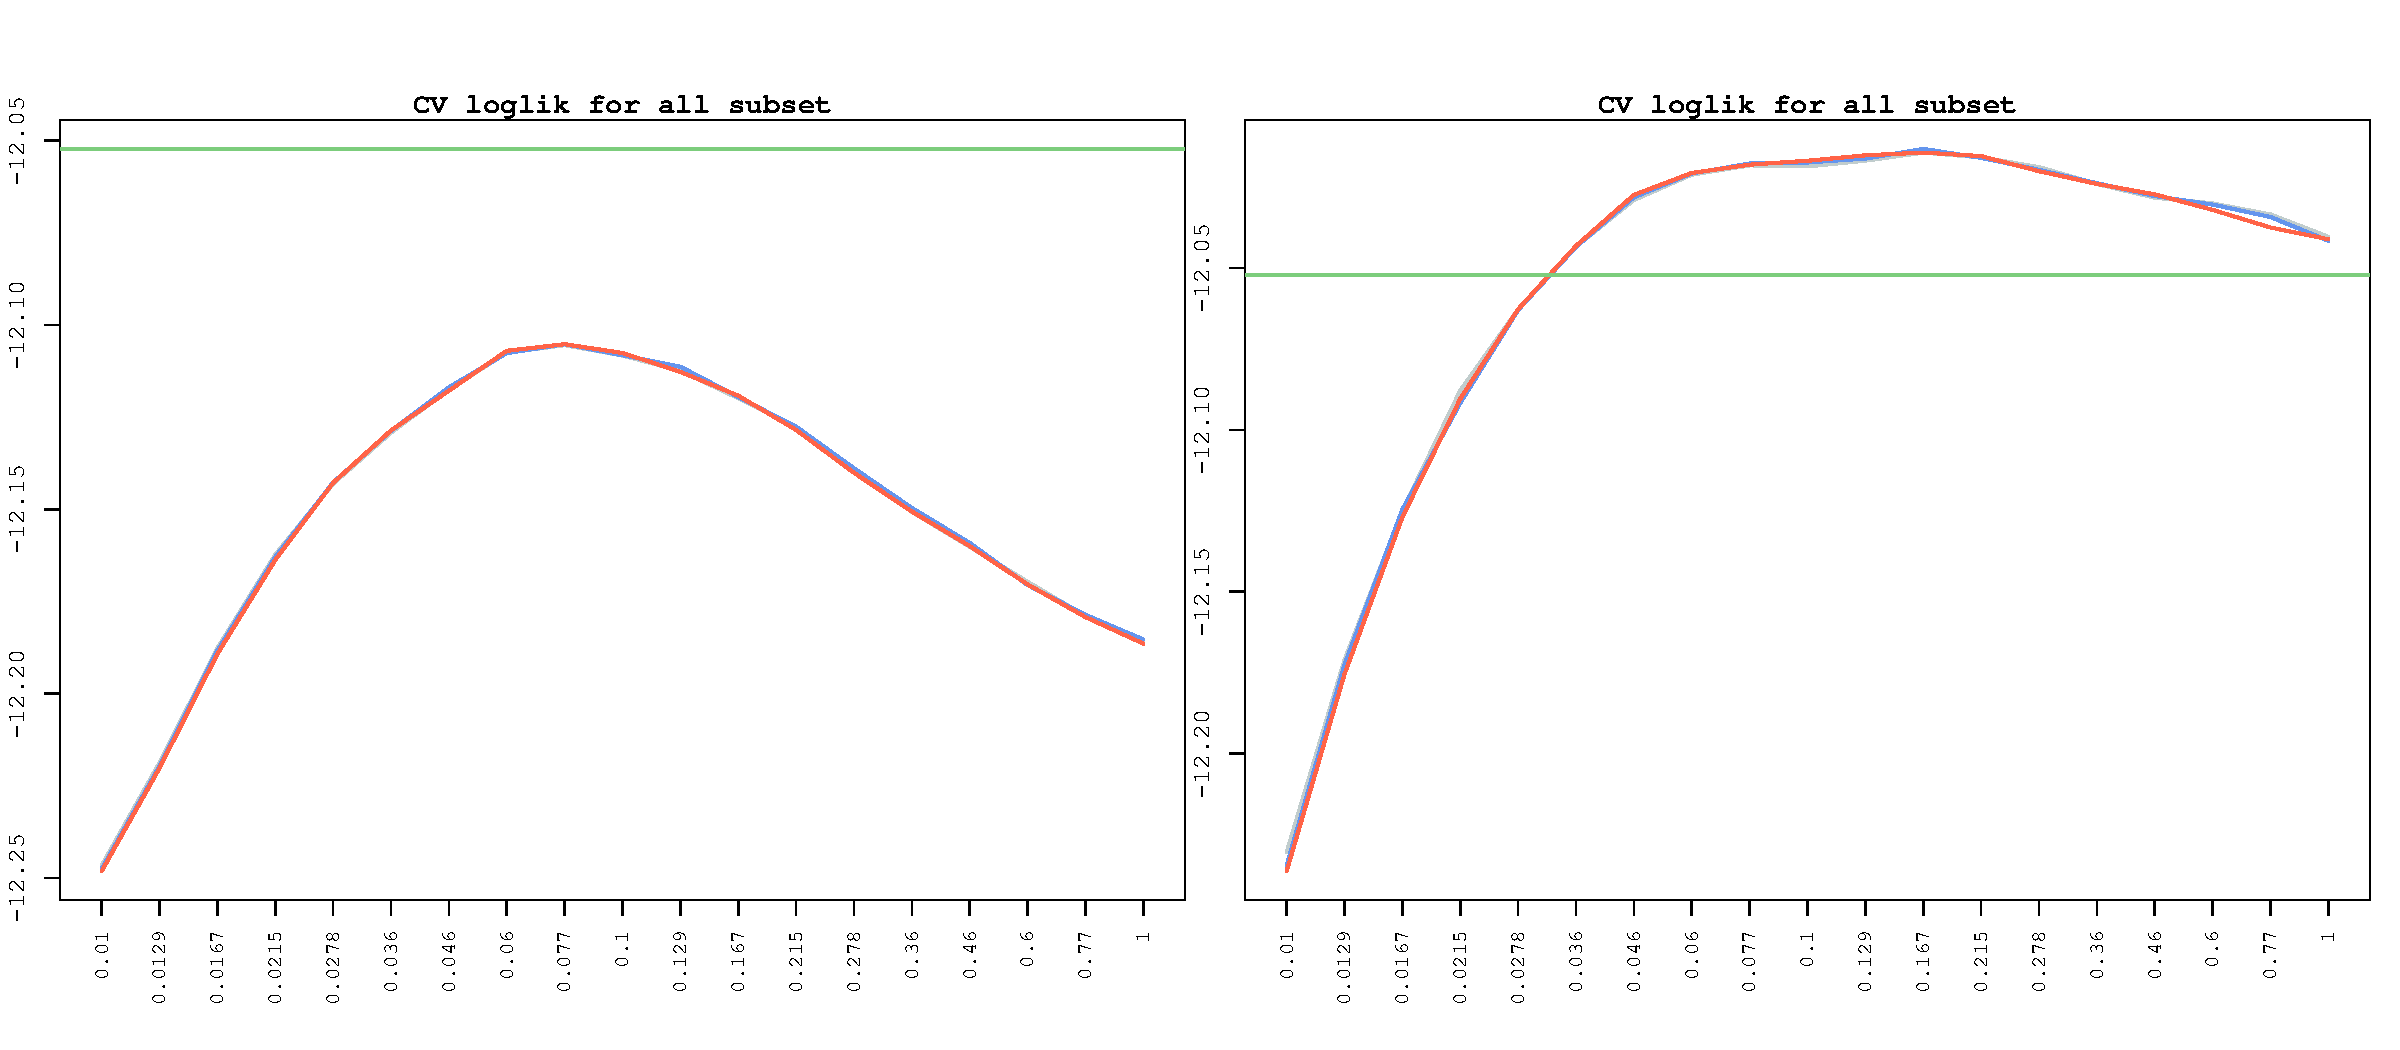
\includegraphics[width=6.5in]{basic.pdf}

%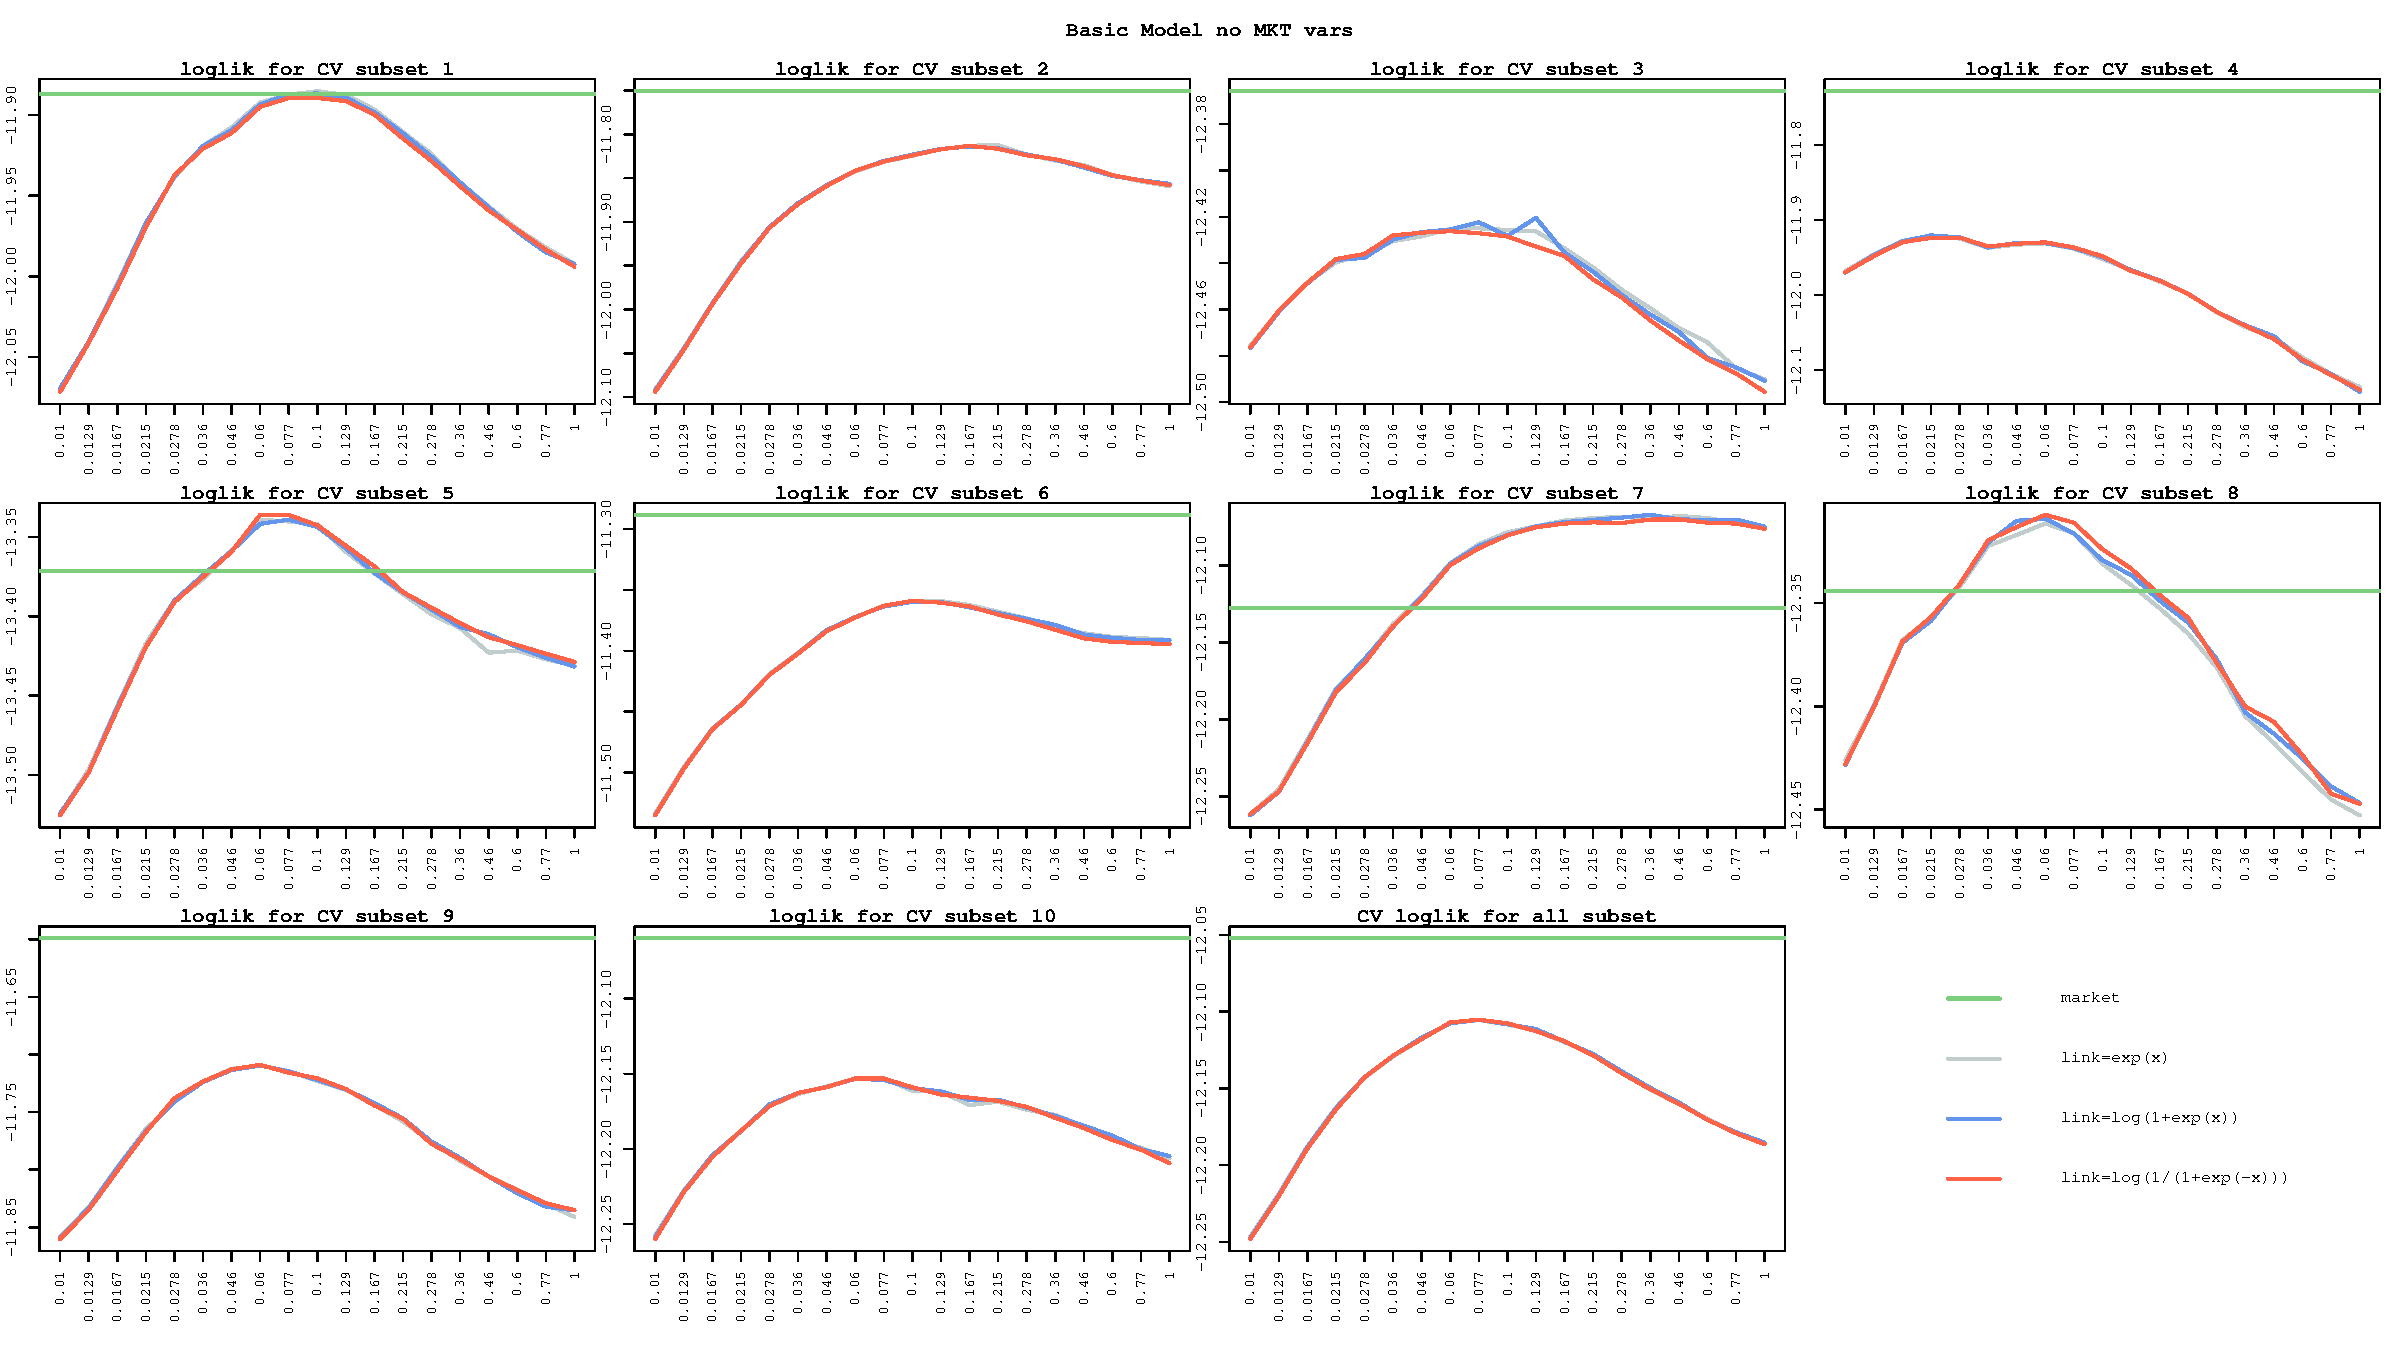
\includegraphics[width=6.5in]{compareBNM.pdf}
%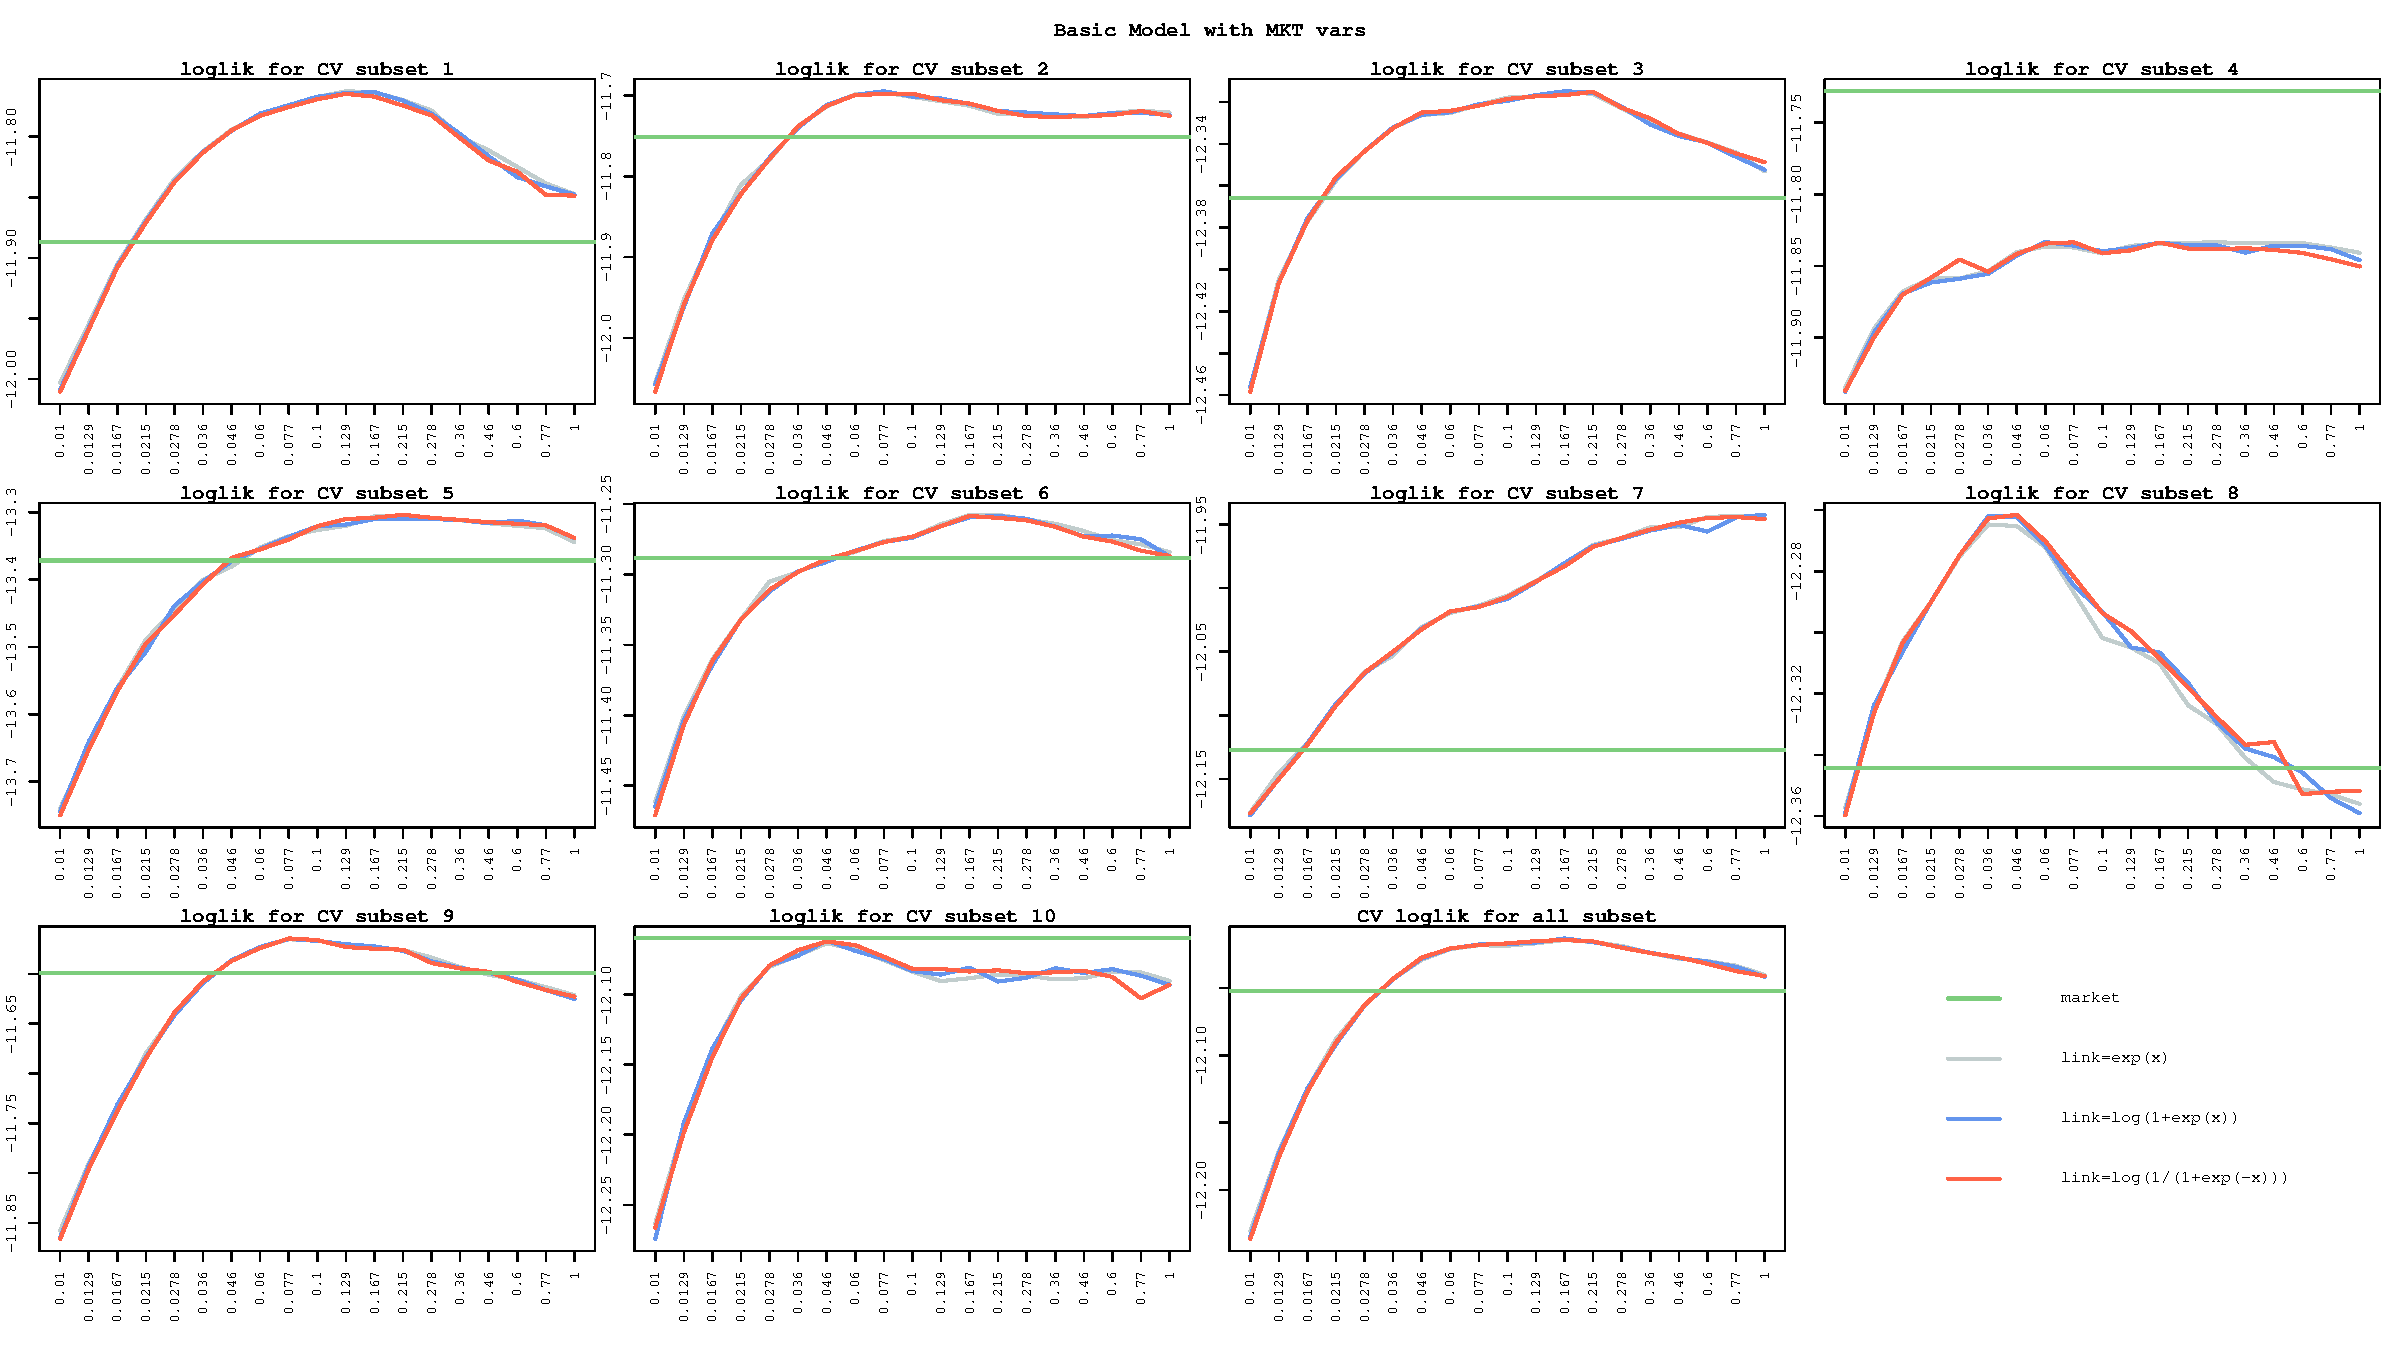
\includegraphics[width=6.5in]{compareBWM.pdf}
 
\newpage
MODEL2: $y_{id}\mid X_{id}, \beta \sim \mathrm{Pois}\zag{\alpha_{i}\lambda_{id}}$

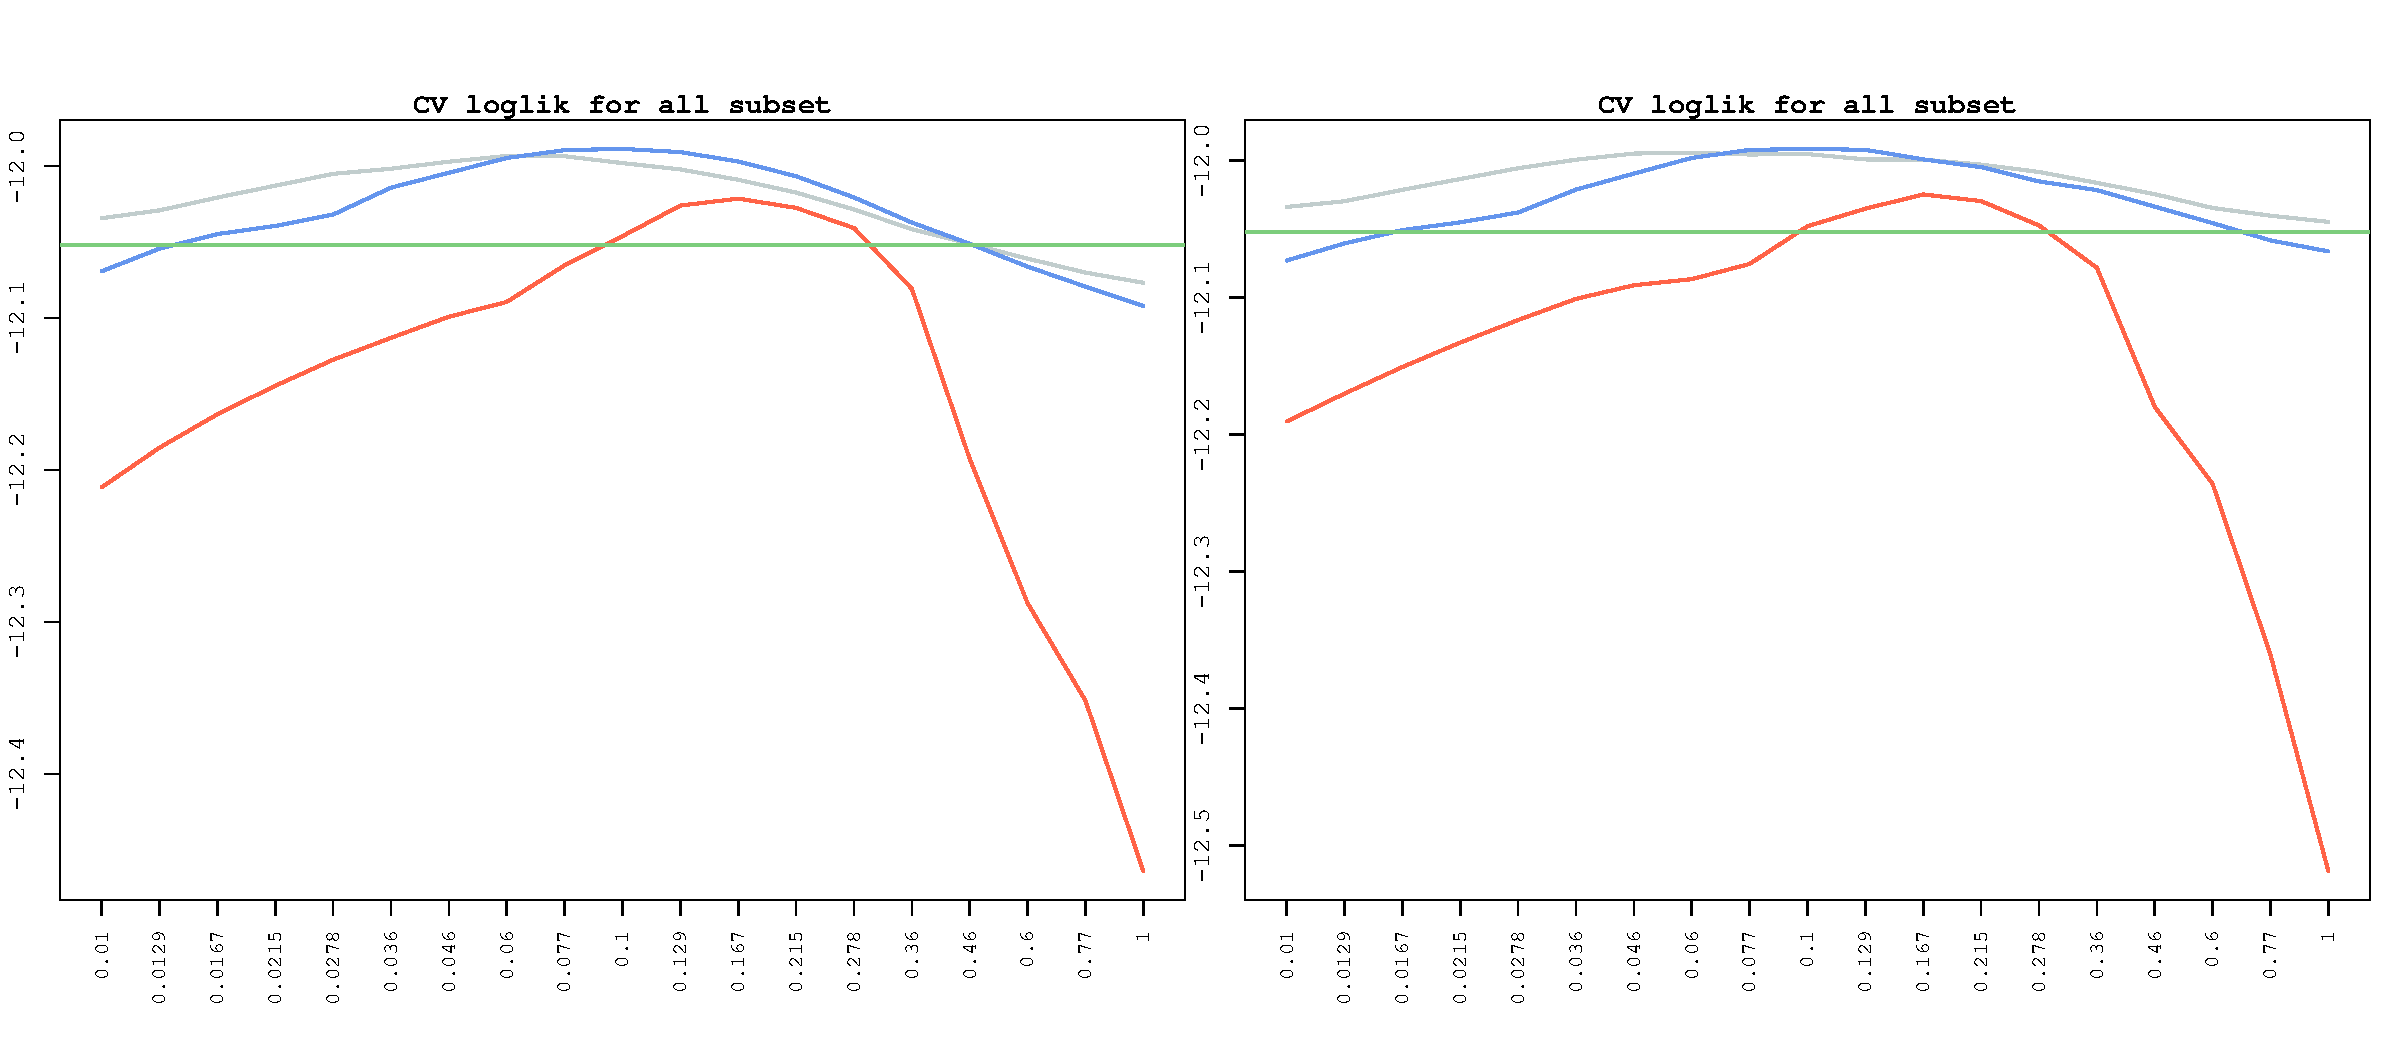
\includegraphics[width=6.5in]{basicMKT.pdf}


%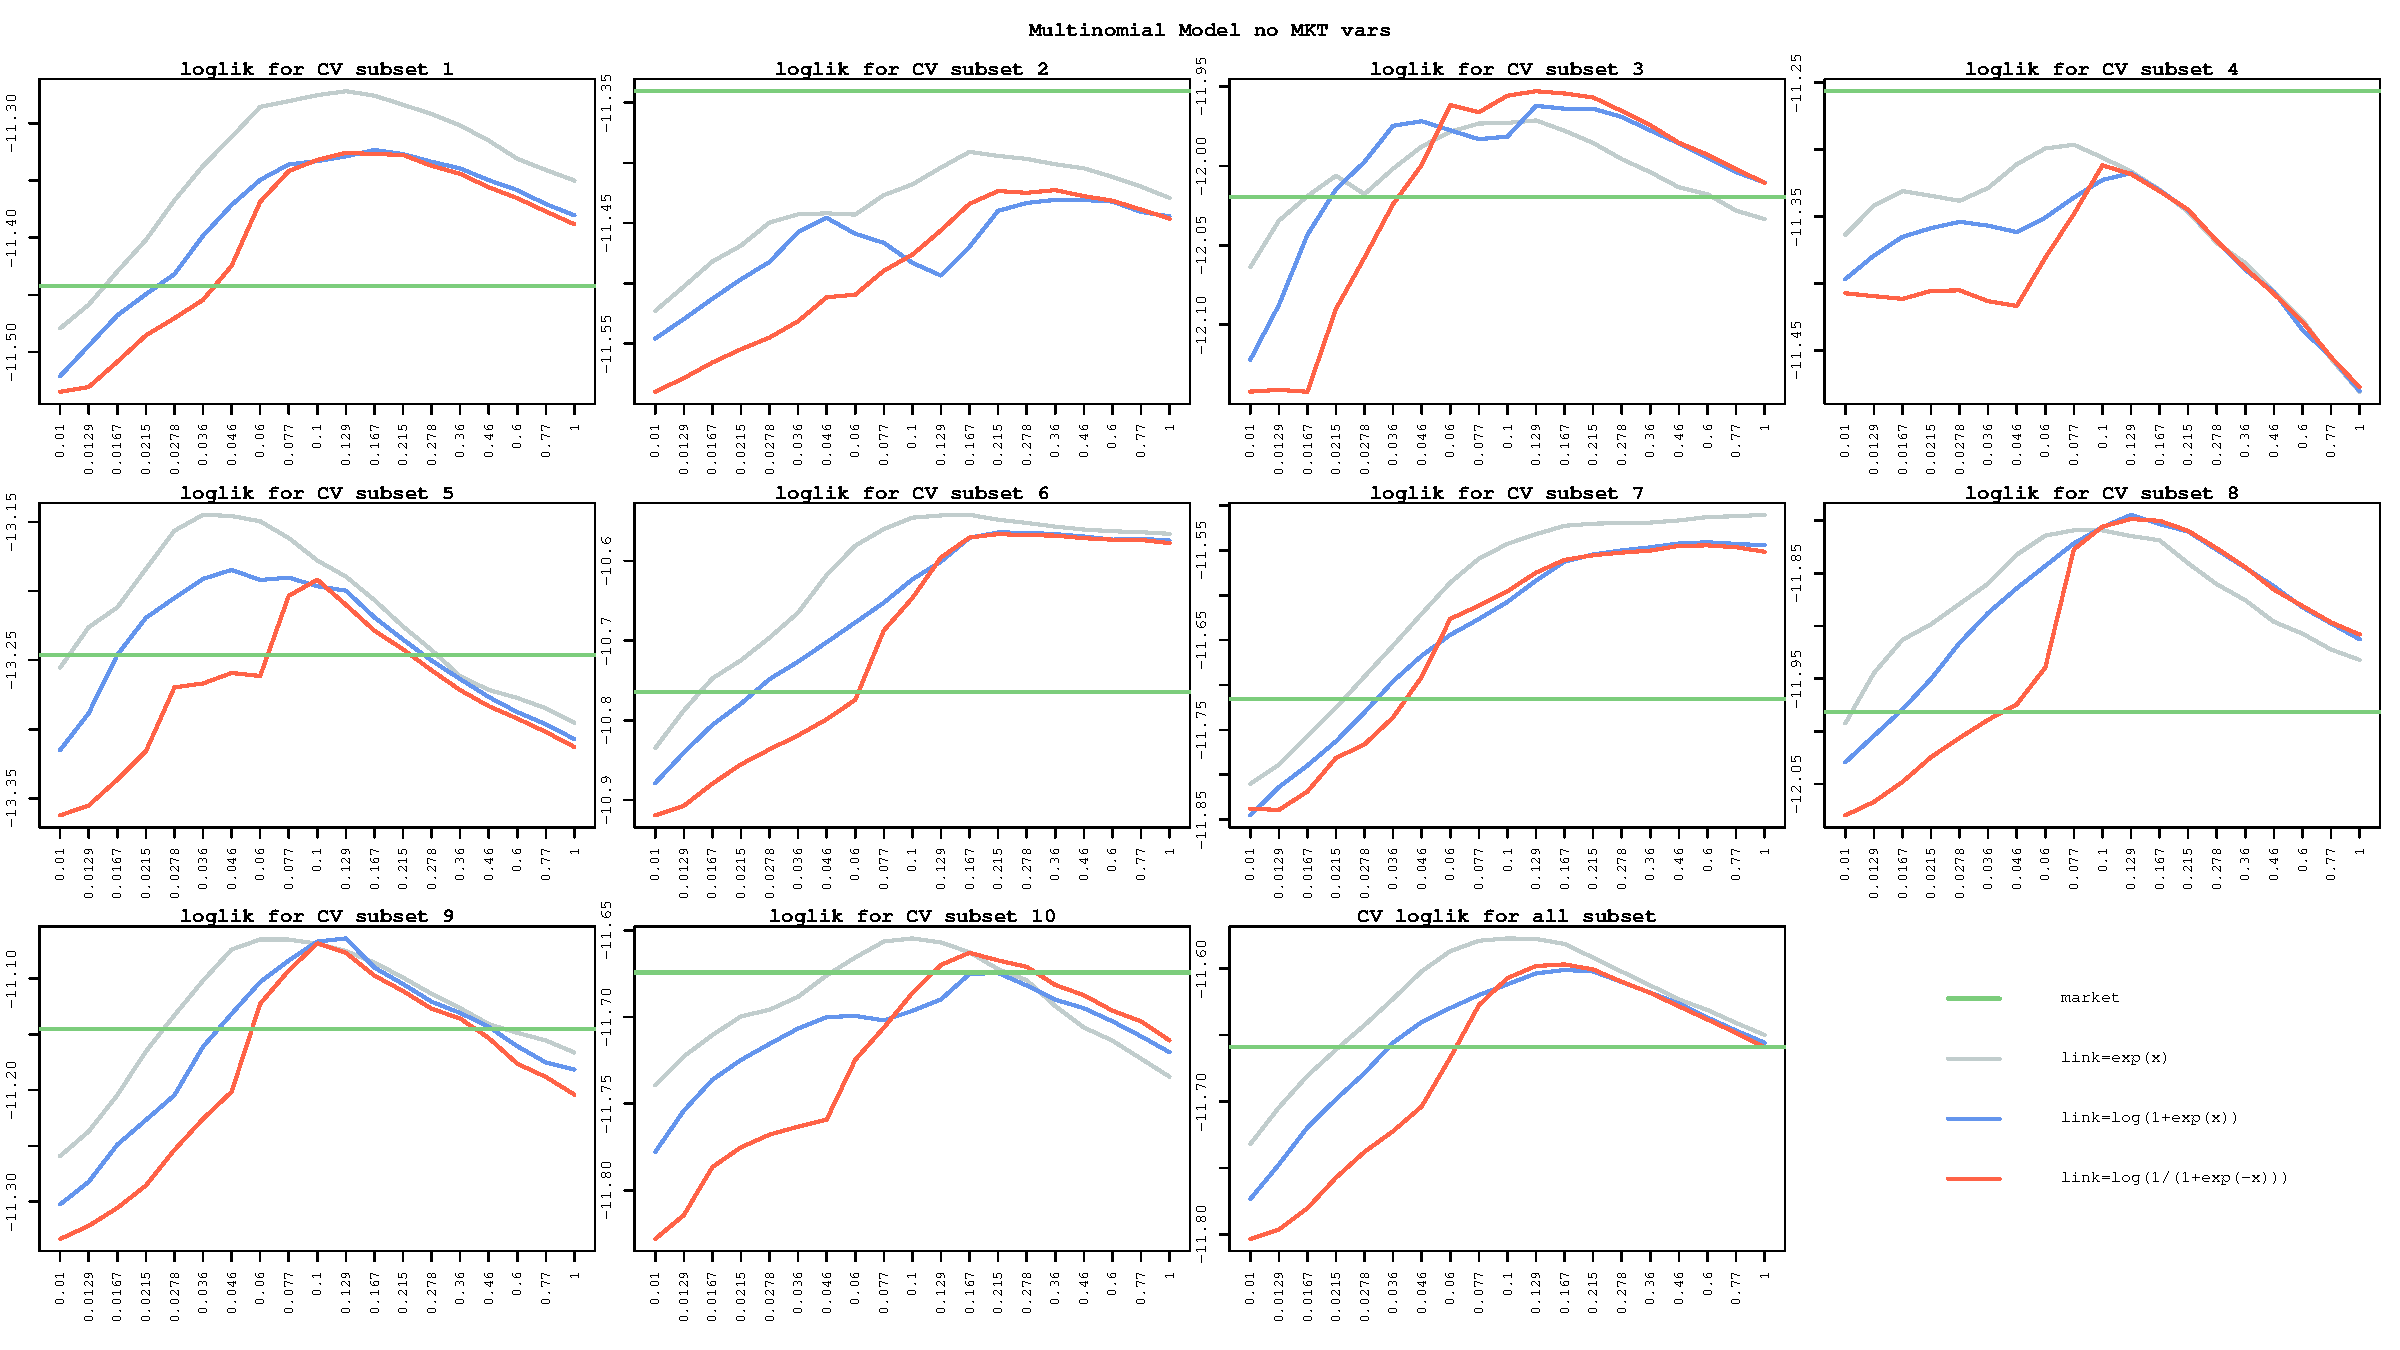
\includegraphics[width=6.5in]{compareBMNM.pdf}
%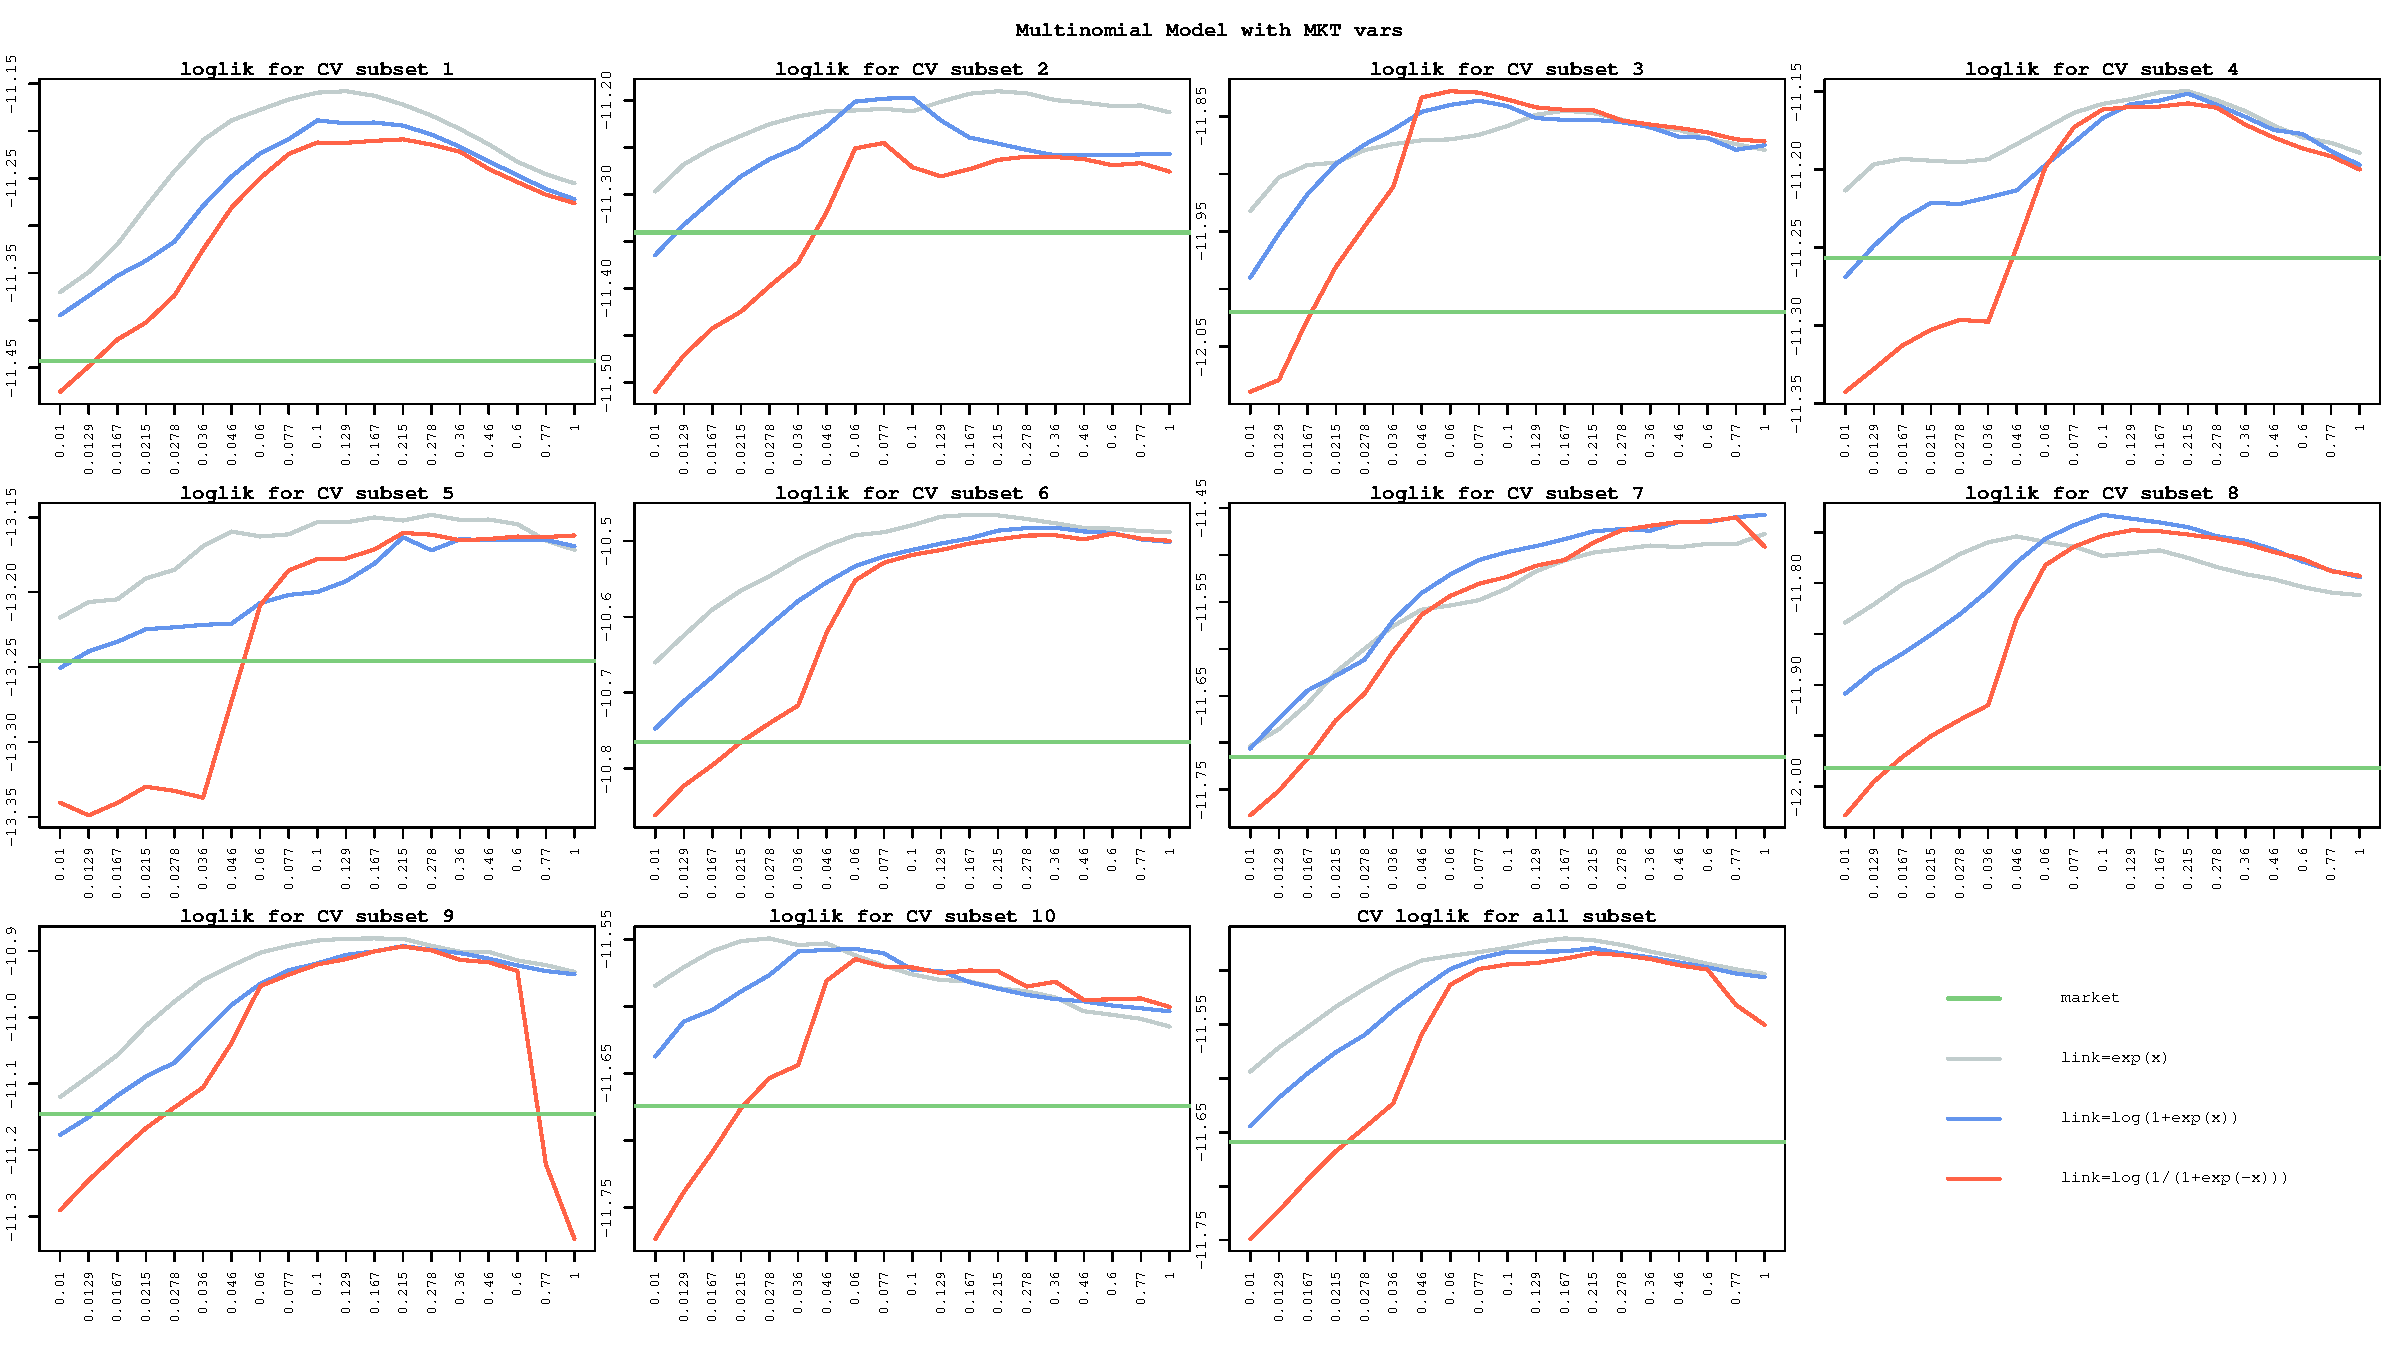
\includegraphics[width=6.5in]{compareBMWM.pdf}

\newpage
MODEL3: $y_{i.}\mid \beta, n_i,  X_{i.}\sim \mathrm{M}
    \zag{n_i, \zagv{\frac{\lambda_{id}}{\sum_{d^\star}\lambda_{id^\star}}}_{d=1}^D}$

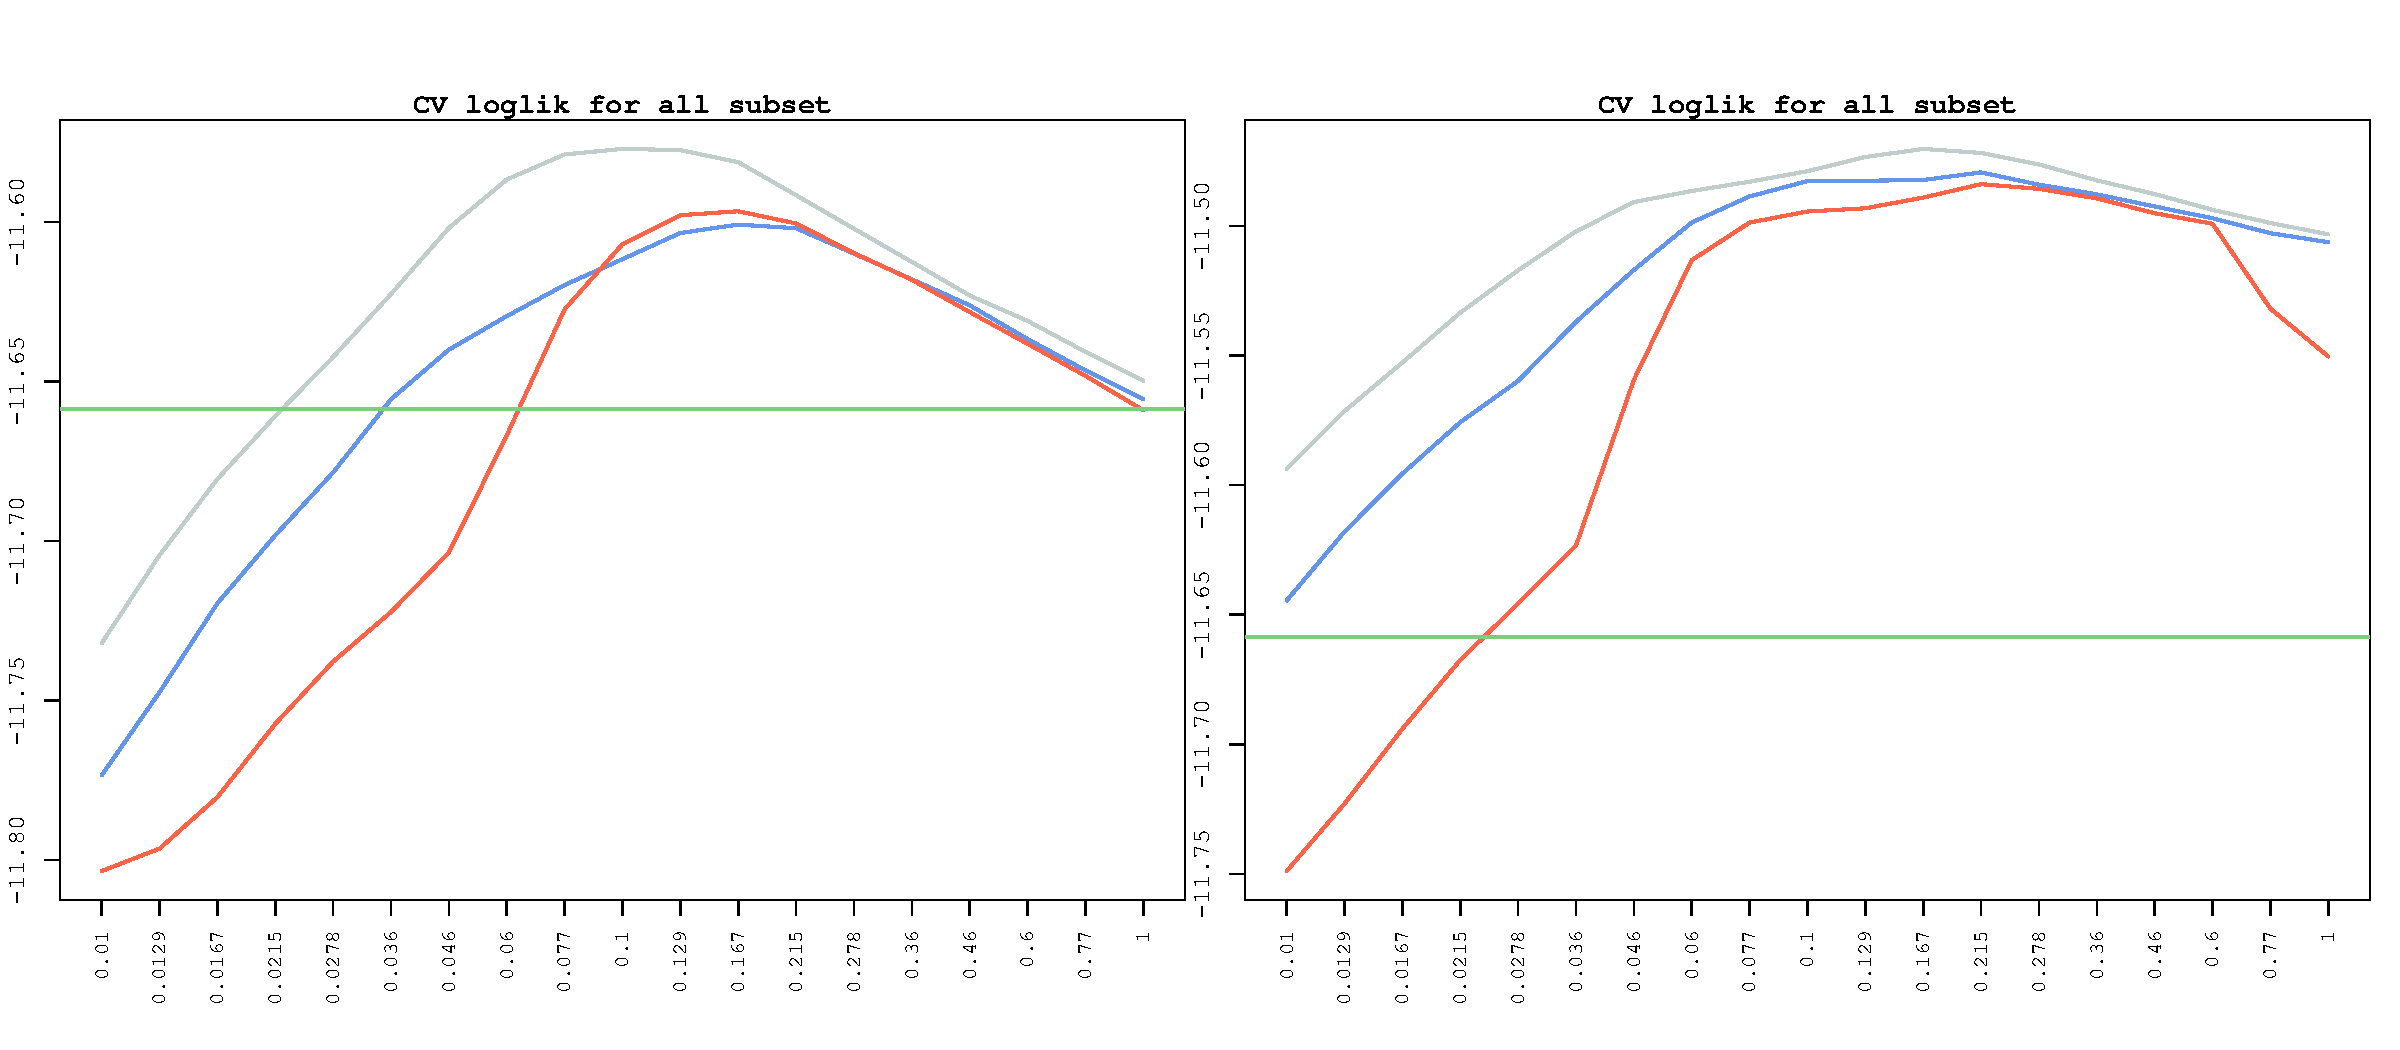
\includegraphics[width=6.5in]{MULT.pdf}

%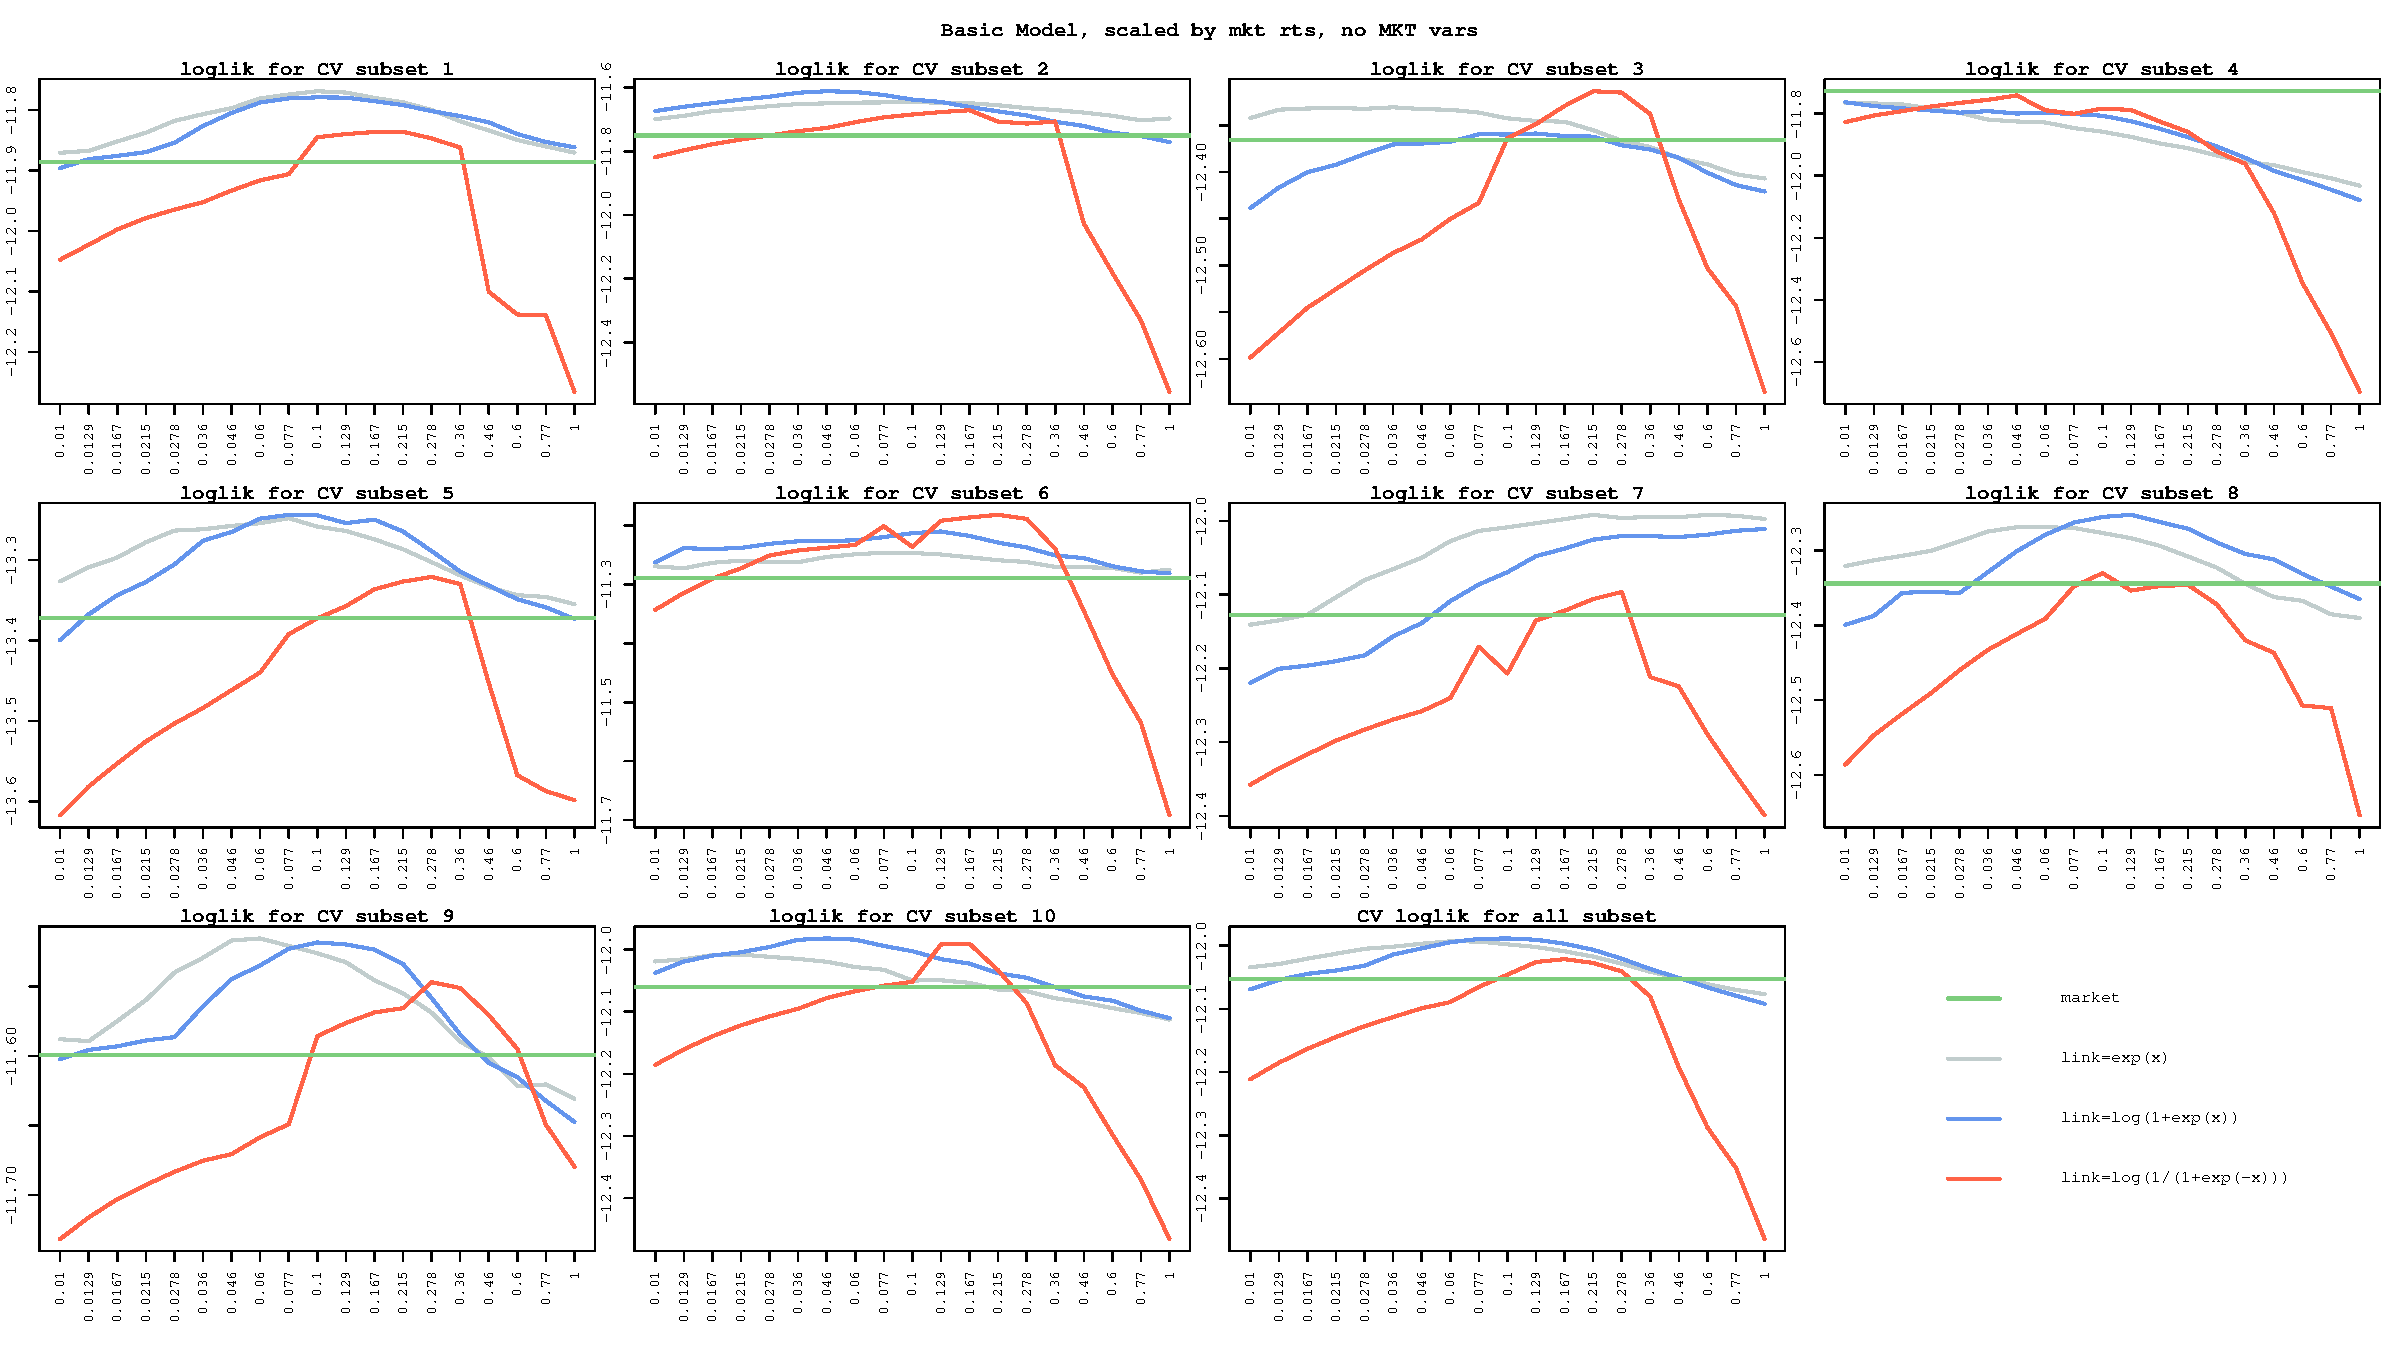
\includegraphics[width=6.5in]{compareMNM.pdf}
%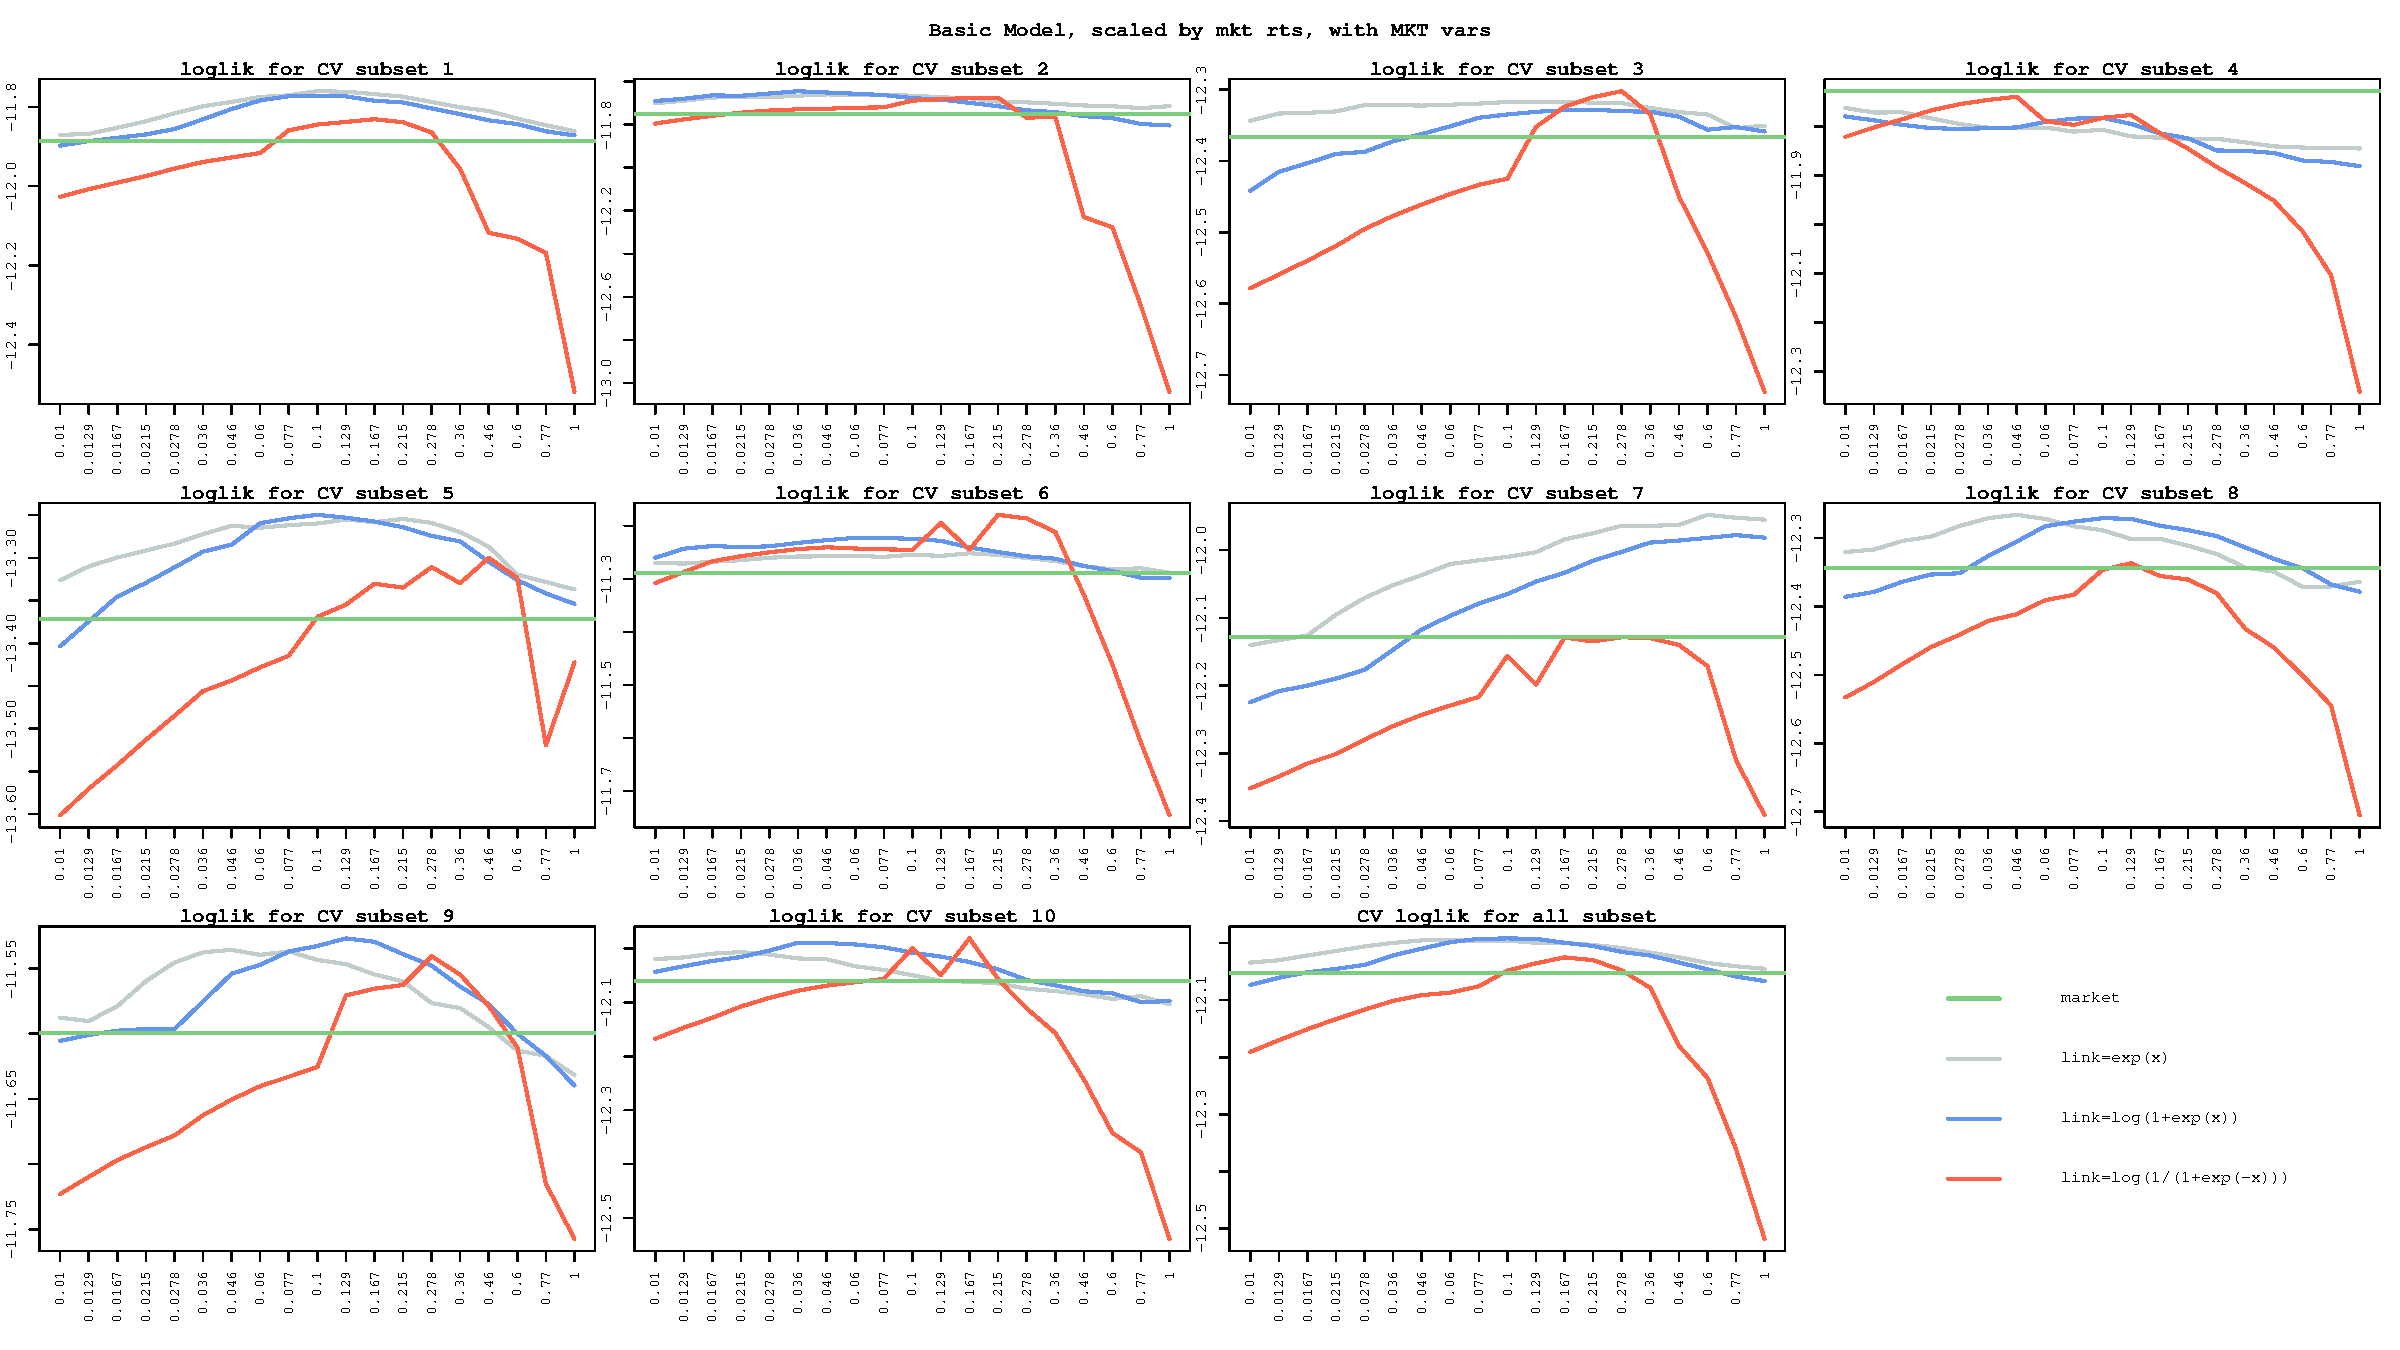
\includegraphics[width=6.5in]{compareMWM.pdf}
%\includegraphics[width=6.5in]{compareMM.pdf}

\newpage

{\LARGE INTRODUCTION: BASIC MODEL}

$$y_{id}\mid X_{id}, \beta \sim \mathrm{Pois}\zag{g(\beta^T X_{id})}$$

$$\mathrm{P}(\beta\mid X, \mathrm{Data}) \propto \mathrm{P}(\beta) \prod_i \prod_d
    g(\beta^T X_{id})^{y_{id}} e^{-g(\beta^T X_{id})}/y_{id}!$$

   -- $d$ are minutes in a match (1-44, 46-89 for both teams; D = 176 per match)\\
   -- $i$ are matches ($I=302$)\\
   -- $g$ is a link function ($\exp(x)$ is default)\\
   -- $K$ number of variables (length of beta)

$$\ell(\beta) = \log(\mathrm{P(\beta)}) + \sum_{l=(i,d)} \zags{y_l\log\zag{g(\beta^T X_l)} - g(\beta^T X_l)} + \mathrm{const}$$

is it convex with respect to beta and lambda???

In coordinatewise gradient descent algorithm in each step $k \in 1,\dots K$ we are maximizing $\ell$ as a function of one parameter $z=\beta_k$. It is fine for convex functions.

So goal is to minimize
$$h(z) = \sum_l \zags{g(r_l + (z-\beta_k)x_{lk}) - y_l\log\zag{g(r_l + (z-\beta_k)x_{lk})}} + z^2/2\tau$$

where $r_l = \beta^T X_l$ and $\tau$ is regularization parameter.

One good way to find the maximum of $\ell$ [David's paper, at al.] is that in each step we find maximum of 2nd degree Tailor polynomial of $h$, so suggested shift for $\beta_k$ will be $\Delta u_k = -h'(\beta_k)/h''(\beta_k)$ where

$$h'(\beta_k) = \sum_l \zags{g'(r_l)x_{lk} - y_l x_{lk} g'(r_l)/g(r_l)} + \beta_k/\tau$$
$$h''(\beta_k) = \sum_l \zags{g''(r_l)x_{lk}^2 - y_l x_{lk}^2 \frac{g''(r_l)g(r_l) - g'(r_l)^2}{g(r_l)^2}} + 1/\tau$$


\newpage
{\LARGE SHAWN'S MODEL}

Pros and cons


$$y_{id}\mid X_{id}, \beta \sim \mathrm{Pois}\zag{\alpha_i g(\beta^T X_{id})}$$

$$P(\beta\mid X, \mathrm{Data}) \propto P(\beta) \prod_i \prod_d
    \zag{\alpha_i g(\beta^T X_{id})}^{y_{id}} e^{-\alpha_i g(\beta^T X_{id})}/y_{id}!$$

Since $n_i = \sum_d y_{id}$ is sufficient statistic for $\alpha_i$ we should maximize

$$P(\beta\mid X, \mathrm{Data}, n) = P(\beta) \prod_i \prod_d
    \zag{\frac{g(\beta^T X_{id})}{\sum_{d^\star}g(\beta^T X_{id^\star})}}^{y_{id}}$$


$$\ell(\beta) = \log(\mathrm{P(\beta)}) + \sum_i \sum_d y_{id}\log{g(\beta^T X_{id})} -
    \sum_i n_i \log {\TS\sum_{d^\star}{g(\beta^T X_{id^\star})}} + \mathrm{const}$$

$$h(z) = \sum_i n_i \log {\TS\sum_{d}{g(r_{id} + (z-\beta_k) x_{idk})}} -
    \sum_{i,d} y_{id}\log{g(r_{id} + (z-\beta_k) x_{idk})} + z^2/2\tau$$

$$h'(\beta_k) = \sum_i n_i \frac{\sum_{d}g'(r_{id})x_{idk}}{\sum_{d} g(r_{id})} -
    \sum_{i,d} y_{id}\frac{g'(r_{id})x_{idk}}{ g(r_{id})} + \beta_k/\tau$$

\begin{equation*}
\begin{split}
h''(\beta_k) = \sum_i n_i& \frac{\zag{\sum_{d}g''(r_{id})x_{idk}^2}\zag{\sum_{d}g(r_{id})} - \zag{\sum_{d}g'(r_{id})x_{idk}}^2 }{\zag{\sum_{d} g(r_{id})}^2} \\ -&
\sum_{i,d} y_{id}x_{idk}^2\frac{g''(r_{id})g(r_{id})- {g'(r_{id})}^2}{{g(r_{id})}^2} + 1/\tau
\end{split}
\end{equation*}

\input{genetic.tex}


\end{document}


\newpage


%\input{relatedwork.tex}

METHODS:

VARIABLE SELECTION:

ALGORITHM:
Explain algorithm like David did (formulas for flexible allowed jump)

Pre-selection of good variables:


DATA:

1. Simulate fake data

2. save data in .Rdata. SoccerSmall1, SoccerSmall2, SoccerLarge1, ..., with or without interactions (double or triple)

3. First 104 variable into txt file and zip and it should  unpack and work

4. prepare different OKs


Fitters:

1. Gradient descent
2. Gradient descent for L1 with flexible allowed jumps (should include part that jumps only if it increases LL)
1. Davids like
2. Mine 1 (fix tau thing -- divide by nvar)
3. Mine 2
4. variable tau fit for forward selection (
fix tau, find best var, fix vars and find best tau, fix tau and find next best var,...)

early stopping of a fitter:

1. if adding new var doesn't improve LL.TE then it is out

2. should record the evolution of the quality of variables, to see if any becomes more important eventually.

EXPERIMENTS:

CODE:

save all interesting output of the fitter into files (condor)

write it to be more clean, prepares and saves data and results automatically (in DAG),

also load data,

loads link functions

maybe:

- have new staring point for beta

- include different tau for for fitter. Finding optimal tau?


RESULTS:

table(L2 basic, L1 basic, L2 Shawn, L1 Shawn, L2 preselected, ..., \\
TR.fit\\
TE.fit\\
time)

1. What is the result of homogenous Poisson (baseline)
2. Can we do better than market
3. Get and plot results from J0 folder. Save into .Rdata
4. for those 20000 fittings find the distributions of non-zero and of zero coefficients. Find (some) score for variables. Make a top list of variables for each tau. Is it different
5.


Picture:

How to check for significance

Saturated link does better?

PDF file for estimates


DISCUSSION:




\begin{itemize}
\item What if you add vars with largest contribution first. Best variables by forward selection could be masked. For example if we add first best then adding next two best variables one-by-one can produce worse results than finding two best at the same time.

\item When adding new best variable optimal $\tau$ can change. What is the best tau as a function of the number of parameters. Probably will be different for L1 and L2. It is decreasing as function of parameters, probably $1/n$ or $1/\sqrt{n}$

\end{itemize}










\end{document}

